\documentclass{article}
\usepackage{graphicx}
\usepackage{epsfig}
%\usepackage{caption}
%\usepackage{subcaption}
\usepackage{epsf}
\usepackage{amssymb}
\usepackage{epstopdf}
\usepackage{amsmath}
\usepackage{braket}
\usepackage{multirow}
\usepackage{array}
\usepackage{mathrsfs}
\usepackage{bm}
\let\vec\bm

\makeatletter
\renewcommand{\fnum@figure}{Fig. \thefigure}
\makeatother

\begin{document}

\title{Cavity-Cavity interaction in the Squeezed Vacuum}
\maketitle 





\section{General master equation of cavity-cavity interaction}
In this section, we consider a scenario where two single-mode leaky cavities are placed inside the waveguide with the squeezed vacuum injected from both ends. The schematic setup is shown in Fig.~\ref{3}. Now we will study how the modes inside the cavity will evolve under the influence of the squeezed vacuum. The free Hamiltonian of cavity and waveguide modes is:
\begin{equation}
\label{eq5a}
\begin{split}
H_{0}=\sum_{i}\hbar\omega(a^{\dagger}a_{i}+\frac{1}{2})+\hbar\sum_{k,s}\omega_{k}(a_{k,s}^{\dagger}a_{k,s}+\frac{1}{2})
\end{split}
\end{equation}
where $a_k$ stands for the mods in the waveguide and $a$ is the field operator of the single mode inside the cavity. The waveguide is saturated with the squeezed vacuum with the center frequency $\omega_0$.  The interaction Hamiltonian between the cavity mode and waveguide modes is:
\begin{equation}
\label{eqa0}
V=-i\hbar\sum_{\vec{k}s}[Da_{\vec{k}s}-D^{+}a_{\vec{k}s}^{\dagger}]
\end{equation}
where
\begin{equation}
\label{eqa1}
\begin{gathered}
 D=\underset{i}{\sum}[g_{i,k,s}^{*}a_{i}^{\dagger}+g_{i,k,s}a_{i}]
\end{gathered}
\end{equation}
Here we define $g_{i,k,s}=|g_{i,k,s}|e^{-ik_z r_i}$ where $r_i$ is just a phenomenological parameter describing the location of cavity. The reduced master equation of atoms in the reservoir is:
\begin{equation}
\label{eqa2}
\begin{split}
\frac{d\rho^{S}}{dt}=&-\frac{1}{\hbar^{2}}\int_{0}^{t}d\tau Tr_{F}\{[V(t),[V(t-\tau),\rho^{S}(t-\tau)\rho^{F}\}\\
=&-\frac{1}{\hbar^{2}}\int_{0}^{t}d\tau Tr_{F}\{V(t)V(t-\tau)\rho^{S}(t-\tau)\rho^{F}+\rho^{S}(t-\tau)\rho^{F}V(t-\tau)V(t)\\
&-V(t)\rho^{S}(t-\tau)\rho^{F}V(t-\tau)-V(t-\tau)\rho^{S}(t-\tau)\rho^{F}V(t)\}.
\end{split}
\end{equation} 

Here we just show how to deal with the first term in Eq.\eqref{eqa2}, the remaining terms can be calculated in the same way. For the first term, we have
\begin{equation}
\label{eqa3}
\begin{split}
&-\frac{1}{\hbar^{2}}\int_{0}^{t}d\tau Tr_{F}\{V(t)V(t-\tau)\rho^{S}(t-\tau)\rho^{F}\}\\
=&\int_{0}^{t}d\tau\underset{\vec{k}s,\vec{k}'s'}{\sum}\{D(t)D(t-\tau)Tr_{F}[\rho^{F}a_{ks}(t)a_{k's'}(t-\tau)]-D(t)D^{+}(t-\tau)Tr_{F}[\rho^{F}a_{ks}(t)a^{\dagger}_{k's'}(t-\tau)]\\
&-D^{+}(t)D(t-\tau)Tr_{F}[\rho^{F}a^{\dagger}_{ks}(t)a_{k's'}(t-\tau)]+D^{+}(t)D^{+}(t-\tau)Tr_{F}[\rho^{F}a^{\dagger}_{ks}(t)a^{\dagger}_{k's'}(t-\tau)]\}\rho^{S}(t-\tau)\}.
\end{split}
\end{equation}
Under the rotating wave approximation(RWA), we have
\begin{equation}
\label{eqa4}
\begin{split}
&-\frac{1}{\hbar^{2}}\int_{0}^{t}d\tau Tr_{F}\{V(t)V(t-\tau)\rho^{S}(t-\tau)\rho^{F}\}\\
=&\sum_{ij}\underset{\vec{k}s,\vec{k'}s'}{\sum}\int_{0}^{t}d\tau\{g_{i,k,s}^{*}a_{i}^{\dagger}e^{i\omega_{i}t}g_{j,k',s'}^{*}a_{j}^{\dagger}e^{i\omega_{j}(t-\tau)}e^{-i(\omega_{\vec{k}s}+\omega_{\vec{k}'s'})t+i\omega_{\vec{k}'s'}\tau}[-\sinh(r)\cosh(r)\delta_{\vec{k}',2\vec{k}_{0}-\vec{k}}\delta_{ss'}]\\
&-g_{i,k,s}^{*}a_{i}^{\dagger}e^{i\omega_{i}t}g_{j,k',s'}a_{j}e^{-i\omega_{j}(t-\tau)}e^{-i\omega_{\vec{k}'s'}\tau}\cosh^{2}r\delta_{\vec{k}\vec{k}'}\delta_{ss'}\\
&-g_{i,k,s}a_{i}e^{-i\omega_{i}t}g_{j,k',s'}^{*}a_{j}^{\dagger}e^{i\omega_{j}(t-\tau)}e^{-i\omega_{\vec{k}'s'}\tau}\cosh^{2}r\delta_{\vec{k}\vec{k}'}\delta_{ss'}\\
&-g_{i,k,s}a_{i}e^{-i\omega_{i}t}g_{j,k',s'}^{*}a_{j}^{\dagger}e^{i\omega_{j}(t-\tau)}e^{i\omega_{\vec{k}'s'}\tau}\sinh^{2}r\delta_{\vec{k}\vec{k}'}\delta_{ss'}\\
&-g_{i,k,s}^{*}a_{i}^{\dagger}e^{i\omega_{i}t}g_{j,k',s'}a_{j}e^{-i\omega_{j}(t-\tau)}e^{i\omega_{\vec{k}'s'}\tau}\sinh^{2}r\delta_{\vec{k}\vec{k}'}\delta_{ss'}\\
&+g_{i,k,s}a_{i}e^{-i\omega_{i}t}g_{j,k',s'}a_{j}e^{-i\omega_{j}(t-\tau)}e^{i(\omega_{\vec{k}s}+\omega_{\vec{k}'s'})t-i\omega_{\vec{k}'s'}\tau}[-\sinh(r)\cosh(r)\delta_{\vec{k}',2\vec{k}_{0}-\vec{k}}\delta_{ss'}]\}\rho^{S}(t-\tau)
\end{split}
\end{equation}
Here we just calculate the first and second term to show how to get the master equation. Define $a$. For the second term, we have
\begin{equation}
\label{eqc2}
\begin{split}
&-\underset{k_{z}}{\sum}\int_{0}^{t}d\tau g_{i,k,s}^{*}a_{i}^{\dagger}e^{i\omega_{i}t}g_{j,k',s'}a_{j}e^{-i\omega_{j}(t-\tau)}e^{-i\omega_{\vec{k}'s'}\tau}\cosh^{2}r\rho^{S}(t-\tau)\delta_{\vec{k}\vec{k}'}\delta_{ss'}\\
=&-\frac{L}{2\pi}e^{i(\omega_{i}-\omega_{j})t}\int_{-\infty}^{\infty}dk_{z}\int_{0}^{t}d\tau e^{i\omega_{j}\tau}e^{-i\omega_{k_{z}}\tau}|g_{i,\vec{k},s}g_{j,\vec{k},s}|e^{ik_{z}(r_{i}-r_{j})}\cosh^{2}ra_{i}^{\dagger}a_{j}\rho^{S}(t-\tau)\\
\approx&-\frac{L}{2\pi}e^{i(\omega_{i}-\omega_{j})t}\int_{0}^{\infty}dk_{z}\int_{0}^{t}d\tau e^{i\omega_{j}\tau}e^{-i[\omega_{j}+c^{2}k_{jz}(k_{z}-k_{jz})/\omega_{j}]\tau}|g_{i,\vec{k},s}g_{j,\vec{k},s}|[e^{ik_{z}(r_{i}-r_{j})}+e^{-ik_{z}(r_{i}-r_{j})}]\cosh^{2}ra_{i}^{\dagger}a_{j}\rho^{S}(t-\tau)\\
\approx&-\frac{L}{2\pi}e^{i(\omega_{i}-\omega_{j})t}\int_{-k_{0z}}^{\infty}d\delta k_{z}\int_{0}^{t}d\tau e^{-i\tau c^{2}k_{jz}\delta k_{z}/\omega_{j}}|g_{i,\vec{k},s}g_{j,\vec{k},s}|[e^{i(k_{jz}+\delta k_{z})(r_{i}-r_{j})}+e^{-i(k_{jz}+\delta k_{z})(r_{i}-r_{j})}]\cosh^{2}ra_{i}^{\dagger}a_{j}\rho^{S}(t-\tau)\\
\approx&-\frac{L}{2\pi}e^{i(\omega_{i}-\omega_{j})t}\int_{-\infty}^{\infty}d\delta k_{z}\int_{0}^{t}d\tau e^{-i(c^{2}k_{jz}\delta k_{z}/\omega_{j})\tau}|g_{i,\vec{k},s}g_{j,\vec{k},s}|[e^{i(k_{jz}+\delta k_{z})(r_{i}-r_{j})}+e^{-i(k_{jz}+\delta k_{z})(r_{i}-r_{j})}]\cosh^{2}ra_{i}^{\dagger}a_{j}\rho^{S}(t-\tau)\\
\approx&-\frac{L}{2\pi}e^{i(\omega_{i}-\omega_{j})t}\int_{0}^{t}d\tau|g_{i,\vec{k},s}g_{j,\vec{k},s}|2\pi[e^{ik_{jz}(r_{i}-r_{j})}\delta((r_{i}-r_{j})-\frac{c^{2}k_{jz}}{\omega_{0}}\tau)+e^{-ik_{jz}(r_{i}-r_{j})}\delta((r_{i}-r_{j})+\frac{c^{2}k_{jz}}{\omega_{0}}\tau)]\cosh^{2}ra_{i}^{\dagger}a_{j}\rho^{S}(t-\tau)\\
\approx&-\frac{L}{2\pi}e^{ik_{jz}r_{ij}}|g_{i,\vec{k},s}g_{j,\vec{k},s}|2\pi\frac{\omega_{j}}{c^{2}k_{0z}}\cosh^{2}ra_{i}^{\dagger}a_{j}\rho^{S}(t)e^{i(\omega_{i}-\omega_{j})t}\\
\approx&-[\frac{\sqrt{\gamma_{i}\gamma_{j}}}{2}\cos(k_{0z}r_{ij})+i\frac{\sqrt{\gamma_{i}\gamma_{j}}}{2}sin(k_{0z}r_{ij})]\cosh^{2}ra_{i}^{\dagger}a_{j}\rho^{S}(t)e^{i(\omega_{i}-\omega_{j})t}\\
\equiv &-(\frac{\sqrt{\gamma_{i}\gamma_{j}}}{2}+i\Lambda_{ij})\cosh^{2}ra_{i}^{\dagger}a_{j}\rho^{S}(t)e^{i(\omega_{i}-\omega_{j})t}
\end{split}
\end{equation}
where $r_{ij}=|r_{i}-r_{j}|$ is also a phenomenological parameter indicating the relative position between cavities. $\gamma_{i}=L|g_{i,k_{0}}|^{2}$ is the leaking rate for the $ith$ cavity, and $\Lambda_{ij}=\sqrt{\gamma_i \gamma_j}\sin(k_{0z}r_{ij})/2$ is the energy shift.
In the third line we expand $\omega_{k}=c\sqrt{(\frac{\pi}{a})^{2}+(k_{z})^{2}}$ around $k_{z}=k_{0z}$ since resonant modes provide dominant contributions. In the fifth line we extend the integration $\int_{-k_{0z}}^{\infty}dk_{z}\rightarrow\int_{-\infty}^{\infty}dk_{z}$ because the main contribution comes from the components around $\delta k_{z}=0$. In the next line, Weisskopf-Wigner approximation is used. %Thus, we have obtained $\gamma_{ij}$ and $\Lambda_{ij}$ as is shown in Eq.\eqref{eq2}. 

Next we need to calculate the first term (squeezing term) in Eq.\eqref{eqa4}:
\begin{equation}
\label{eqb8}
\begin{split}
& e^{i(\omega_{i}+\omega_{j}-2\omega_{0})t}\underset{k_{z}}{\sum}\int_{0}^{t}d\tau\{g_{i,2\vec{k}_{0}-\vec{k}}^{*}a_{i}^{\dagger}g_{j,\vec{k}}^{*}a_{j}^{\dagger}e^{i(\omega_{\vec{k}}-\omega_{j})\tau}[-\sinh(r)\cosh(r)]\rho^{S}(t-\tau) \\
&=-\frac{L}{2\pi}e^{i(\omega_{i}+\omega_{j}-2\omega_{0})t}\int_{0}^{2k_{0z}}dk_{z}\int_{0}^{t}d\tau e^{i(\omega_{k_{z}}-\omega_{j})\tau}e^{i(2k_{iz}-k_{z})(r_{i}-o_{1})}e^{ik_{z}(r_{j}-o_{1})}|g_{i,2\vec{k}_{0}-\vec{k}}g_{j,\vec{k}}|\sinh(r)\cosh(r)a_{i}^{\dagger}a_{j}^{\dagger}\rho^{S}(t-\tau)\\ 
&-\frac{L}{2\pi}e^{i(\omega_{i}+\omega_{j}-2\omega_{0})t}\int_{-2k_{0z}}^{0}dk_{z}\int_{0}^{t}d\tau e^{i(\omega_{k_{z}}-\omega_{j})\tau}e^{i(-2k_{iz}-k_{z})(r_{i}-o_{2})}e^{ik_{z}(r_{j}-o_{2})}|g_{i,2\vec{k}_{0}-\vec{k}}g_{j,\vec{k}}|\sinh(r)\cosh(r)a_{i}^{\dagger}a_{j}^{\dagger}\rho^{S}(t-\tau)
\end{split}
\end{equation}
Putting the overall factor $e^{i(\omega_i+\omega_j-2\omega_0)t}$ aside, for $i=j$, Eq.\eqref{eqb8} reduces to 
\begin{equation}
\label{eqb9}
\begin{split}
&\underset{k_{z}}{\sum}\int_{0}^{t}d\tau\{g_{i,2\vec{k}_{0}-\vec{k}}^{*}a_{i}^{\dagger}g_{i,\vec{k}}^{*}a_{i}^{\dagger}e^{i(\omega_{\vec{k}}-\omega_{i})\tau}[-\sinh(r)\cosh(r)]\rho^{S}(t-\tau)\\
&=-\frac{L}{2\pi}\int_{0}^{2k_{0z}}dk_{z}\int_{0}^{t}d\tau e^{i\frac{c^{2}k_{iz}}{_{\omega_{i}}}(k_{z}-k_{iz})\tau}e^{i2k_{0z}(r_{i}-o_{1})}|g_{i,2\vec{k}_{0}-\vec{k}}g_{i,\vec{k}}|\sinh(r)\cosh(r)a_{i}^{\dagger}a_{i}^{\dagger}\rho^{S}(t-\tau)\\
&-\frac{L}{2\pi}\int_{-2k_{0z}}^{0}dk_{z}\int_{0}^{t}d\tau e^{i\frac{c^{2}k_{iz}}{_{\omega_{i}}}(k_{z}-k_{iz})\tau}e^{-i2k_{0z}(r_{i}-o_{2})}|g_{i,2\vec{k}_{0}-\vec{k}}g_{i,\vec{k}}|\sinh(r)\cosh(r)a_{i}^{\dagger}a_{i}^{\dagger}\rho^{S}(t-\tau)\\
&=-\frac{L}{2\pi}[e^{i2k_{0z}(r_{i}-o_{1})}+e^{-i2k_{0z}(r_{i}-o_{2})}]|g_{i,2\vec{k}_{0}-\vec{k}}g_{i,\vec{k}}|\int_{0}^{t}d\tau2\pi\delta(\frac{c^{2}k_{iz}}{\omega_{i}}\tau)\sinh(r)\cosh(r)a_{i}^{\dagger}a_{i}^{\dagger}\rho^{S}(t-\tau)\\
& =-e^{i2k_{0z}R}\frac{\gamma_{i}}{2}\cos(2k_{0z}r_{i})\sinh(r)\cosh(r)a_{i}^{\dagger}a_{i}^{\dagger}\rho^{S}(t)
\end{split}
\end{equation}
where we have used the fact that the origin of coordinate system is at equal distant from two sources(i.e., $o_2=-o_1=R$) in the second last line. Thus, we have $\gamma'_{ij}=\sqrt{\gamma_{i}\gamma_{j}}\cos(2k_{0z}r_{i})$. For $r_i\neq r_j$, Eq. \eqref{eqb8} reduces to
\begin{equation}
\label{eqb10}
\begin{split}
&\underset{k_{z}}{\sum}\int_{0}^{t}d\tau\{g_{i,2\vec{k}_{0}-\vec{k}}a_{i}^{\dagger}g_{j,\vec{k}}a_{j}^{\dagger}e^{i(\omega_{\vec{k}}-\omega_{j})\tau}[-\sinh(r)\cosh(r)]\rho^{S}(t-\tau)\\
&=-\frac{L}{2\pi}\int_{0}^{2k_{0z}}dk_{z}\int_{0}^{t}d\tau e^{i\frac{c^{2}k_{jz}}{_{\omega_{j}}}(k_{z}-k_{jz})\tau}e^{i2k_{0z}(r_{c}-o_{1})}e^{-i(k_{z}-k_{0z})(r_{i}-r_{j})}|g_{i,2\vec{k}_{0}-\vec{k}}g_{j,\vec{k}}|\sinh(r)\cosh(r)a_{i}^{\dagger}a_{j}^{\dagger}\rho^{S}(t-\tau)\\
& -\frac{L}{2\pi}\int_{-2k_{0z}}^{0}dk_{z}\int_{0}^{t}d\tau e^{i\frac{c^{2}k_{jz}}{_{\omega_{j}}}(-k_{z}-k_{jz})\tau}e^{-i2k_{0z}(r_{c}-o_{2})}e^{-i(k_{z}+k_{0z})(r_{i}-r_{j})}|g_{i,2\vec{k}_{0}-\vec{k}}g_{j,\vec{k}}|\sinh(r)\cosh(r)a_{i}^{\dagger}a_{j}^{\dagger}\rho^{S}(t-\tau)\\
&=-\frac{L}{2\pi}e^{i2k_{0z}(r_{c}-o_{1})}|g_{i,2\vec{k}_{0}-\vec{k}}g_{j,\vec{k}}|\int_{-\infty}^{\infty}dk_{z}\int_{0}^{t}d\tau e^{i\frac{c^{2}k_{jz}}{_{\omega_{j}}}(k_{z}-k_{jz})\tau}e^{-i(k_{z}-k_{0z})(r_{i}-r_{j})}\sinh(r)\cosh(r)a_{i}^{\dagger}a_{j}^{\dagger}\rho^{S}(t-\tau) \\
& -\frac{L}{2\pi}e^{-i2k_{0z}(r_{c}-o_{2})}|g_{i,2\vec{k}_{0}-\vec{k}}g_{j,\vec{k}}|\int_{-\infty}^{\infty}dk_{z}\int_{0}^{t}d\tau e^{i\frac{c^{2}k_{jz}}{_{\omega_{j}}}(k_{z}-k_{jz})\tau}e^{i(k_{z}-k_{0z})(r_{i}-r_{j})}\sinh(r)\cosh(r)a_{i}^{\dagger}a_{j}^{\dagger}\rho^{S}(t-\tau) \\
& \approx-\frac{L}{2\pi}e^{i2k_{0z}R}|g_{i,2\vec{k}_{0}-\vec{k}}g_{j,\vec{k}}|\int_{0}^{t}d\tau2\pi[e^{i2k_{0z}r_{c}}\delta(r_{i}-r_{j}-\frac{c^{2}k_{0z}}{_{\omega_{0}}}\tau)+e^{-i2k_{0z}r_{c}}\delta(r_{i}-r_{j}+\frac{c^{2}k_{0z}}{_{\omega_{0}}}\tau)]\sinh(r)\cosh(r)a_{i}^{\dagger}a_{j}^{\dagger}\rho^{S}(t-\tau)\\
&\approx-e^{i2k_{0z}R}L|g_{i,2\vec{k}_{0}}g_{j,\vec{k}_{0}}|e^{i2k_{0z}r_{c}sgn(i-j)}a_{i}^{\dagger}a_{j}^{\dagger}\rho^{S}(t)\rightarrow-\frac{\sqrt{\gamma_{i}\gamma_{j}}}{2}e^{i2k_{0z}R}\cos(k_{0z}(r_{i}+r_{j}))a_{i}^{\dagger}a_{j}^{\dagger}\rho^{S}(t)\\
\end{split}
\end{equation}
where $sgn(i-j)$ is the sign function. The last arrow is because we need to sum over $i,j$, so the imaginary part of $e^{i2k_{0z}r_{c}sgn(i-j)}$ vanishes and the neat result is that $\gamma'_{ij}=e^{i2k_{0z}R}\sqrt{\gamma_{i}\gamma_{j}}\cos(k_{0z}(r_{i}+r_{j}))$. As for $a_{i}^{\dagger}\rho^{S}(t)a_{j}^{\dagger}$ terms, the combination of the last two terms in Eq.\eqref{eqa2} will make the imaginary part of $e^{i2k_{0z}r_{c}sgn(i-j)}$ vanish. Thus, we have $\gamma'_{ij}=e^{i2k_{0z}R}\sqrt{\gamma_{i}\gamma_{j}}\cos(k_{0z}(r_i+r_j))$. If one needs to get $\gamma_{ij}, \gamma'_{ij}$ and $\Lambda_{ij}$in the unidirectional waveguide case, we just need to discard the second terms in the parenthesis of Eq.\eqref{eqc2} and Eq.\eqref{eqb10}.



\begin{figure*}
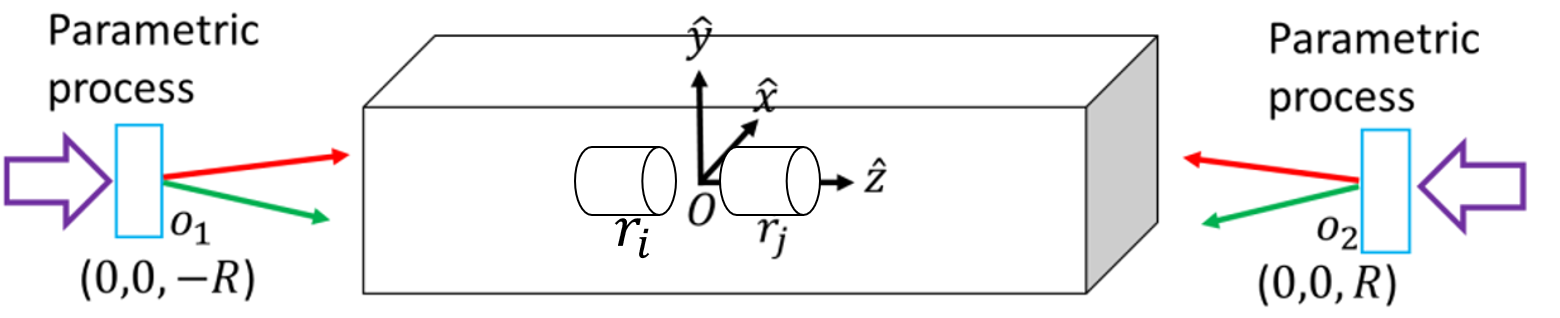
\includegraphics[width=0.8\columnwidth]{fig3.png}
\caption{(a) Schematic setup: two single-mode cavities are placed inside the waveguide with the broadband squeezed vacuum incident from both ends.}
\label{3}
\end{figure*}

Thus, the general equation for cavity-cavity interaction in the squeezed vacuum is:
\begin{equation}
\label{eq0}
\begin{split}
\dot{\rho}&=\sum_{ij}\gamma\cosh^{2}r(-\rho a_{i}^{\dagger}a_{j}-a_{i}^{\dagger}a_{j}\rho+2a_{i}\rho a_{j}^{\dagger})\\
&+\gamma\sinh^{2}r(-\rho a_{i}a_{j}^{\dagger}-a_{i}a_{j}^{\dagger}\rho+2a_{i}^{\dagger}\rho a_{j})\\
&+\gamma\cosh r\sinh r(e^{i\theta}\rho a_{i}a_{j}+e^{i\theta_{i}}a_{i}a_{j}\rho-e^{i\theta}2a_{i}\rho a_{j}+h.c.)\\
\end{split}
\end{equation}
First, we study two non-resonant cavities coupled to the squeezed vacuum reservoir. The eigen frequencies of these two cavities are $\omega_1=\omega_0-\delta \omega$ and $\omega_2=\omega_0+\delta \omega$, following exacly the same steps as the derivation in Appendix A with $S$ replaced by $a_k$, we get:
\begin{equation}
\label{eq6}
\begin{split}
\dot{\rho}&=\sum_{i}\gamma(1+N)(-\rho a_{i}^{\dagger}a_{i}-a_{i}^{\dagger}a_{i}\rho+2a_{i}\rho a_{i}^{\dagger})\\
&+\gamma N(-\rho a_{i}a_{i}^{\dagger}-a_{i}a_{i}^{\dagger}\rho+2a_{i}^{\dagger}\rho a_{i})\\
&+\sum_{i\ne j}\gamma M(e^{i\theta}\rho a_{i}a_{j}+e^{i\theta}a_{i}a_{j}\rho-2e^{i\theta}a_{i}\rho a_{j}+h.c.)\\
\end{split}
\end{equation}
where $\theta$ is a phase factor which depends on the relative position of cavities and the squeezing source. The above equation can be re-arranged as:
\begin{equation}
\label{eq7}
\begin{split}
\dot{\rho}&=\sum_{i\ne j}\frac{\gamma}{2}[-\rho(\cosh(r)a_{i}^{\dagger}-e^{i\theta}\sinh(r)a_{j})(\cosh(r)a_{i}-e^{-i\theta}\sinh(r)a_{j}^{\dagger})\\
&-(\cosh(r)a_{i}^{\dagger}-e^{i\theta}\sinh(r)a_{j})(\cosh(r)a_{i}-e^{-i\theta}\sinh(r)a_{j}^{\dagger})\rho\\
&+2(\cosh(r)a_{i}-e^{-i\theta}\sinh(r)a_{j}^{\dagger})\rho(\cosh(r)a_{i}^{\dagger}-e^{i\theta}\sinh(r)a_{j})]
\end{split}
\end{equation}
we use the following Bogoliubov transformation\cite{Bogoliubov}:
\begin{equation}
\label{eq8}
\begin{split}
&S=exp(\eta^{\star}a_{i}a_{j}-\eta a_{i}^{\dagger}a_{j}^{\dagger})\\
&A_{i}=S^{+}a_{i}S=\cosh(r)a_{i}-e^{-i\theta}\sinh(r)a_{j}^{\dagger} \\
&A_{i}^{+}=S^{+}a_{i}^{+}S=\cosh(r)a_{i}^{+}-e^{i\theta}\sinh(r)a_{j}\\
\end{split}
\end{equation}
so the master equation Eq.\eqref{eq7} becomes:
\begin{equation}
\label{eq9}
\begin{split}
\dot{\rho}=\sum_{i}\gamma[-\rho A_{i}^{\dagger}A_{i}-A_{i}^{\dagger}A_{i}\rho+2A_{i}\rho A_{i}^{\dagger}]
\end{split}
\end{equation}
Next we redefine the density matrix: $\rho_{s}=S\rho S^{\dagger}$. Thus Eq.\eqref{eq9} becomes:
\begin{equation}
\label{eq11}
\begin{split}
\dot{\rho}_{s}&=\sum_{i}\gamma[-\rho_{s}a_{i}^{\dagger}a_{i}-a_{i}^{\dagger}a_{i}\rho_{s}+2a_{i}\rho_{s}a_{i}^{\dagger}]\\
&\equiv\sum_{i}\gamma[-a_{i}^{l\dagger}a_{i}^{l}\rho_{s}-a_{i}^{r\dagger}a_{i}^{r}\rho_{s}+2a_{i}^{r}a_{i}^{l\dagger}\rho_{s}]\equiv L\rho_{s}
\end{split}
\end{equation}
Here we define superoperator $\{a_{i}^{l}, a_{i}^{l\dagger}\}$($\{a_{i}^{r}, a_{r}^{l\dagger}\}$ ) only acting to the left(right) on density operator $\rho$ \cite{Wang2002, An}. These operators have the following commutation relations: 
\begin{equation}
\label{eq12}
\begin{split}
[a_{i}^{r},a_{j}^{r\dagger}]=\delta_{ij},\,[a_{i}^{l},a_{j}^{l\dagger}]=-\delta_{ij},\,[a_{i}^{l},a_{j}^{r\dagger}]=[a_{i}^{l},a_{j}^{r}]=[a_{i}^{l\dagger},a_{j}^{r}]=[a_{i}^{l\dagger},a_{j}^{r\dagger}]=0
\end{split}
\end{equation}
Thus, the steady state of Eq.\eqref{eq11} can be solved by solving $L\rho=0$, which requires the diagnolization of superoperator $L$. Applying the similarity transformation $U=e^{-a_{1}^{r}a_{1}^{l\dagger}-a_{2}^{r}a_{2}^{l\dagger}}$ to Eq.\eqref{eq11} , since we have $U^{-1}(a_{i}^{r\dagger},a_{i}^{l},a_{i}^{r},a_{i}^{l\dagger})U=(a_{i}^{r\dagger}+a_{i}^{l\dagger},a_{i}^{r}+a_{i}^{l},a_{i}^{r},a_{i}^{l\dagger})$, the right hand side of Eq.\eqref{eq11} becomes:
\begin{equation}
\label{eq13}
\begin{split}
RHS=\sum_{i}\gamma U^{-1}[-a_{i}^{l\dagger}a_{i}^{l}-a_{i}^{r\dagger}a_{i}^{r}+2a_{i}^{r}a_{i}^{l\dagger}]UU^{-1}\rho_{s}=\sum_{i}\gamma[-a_{i}^{l\dagger}a_{i}^{l}-a_{i}^{r\dagger}a_{i}^{r}]U^{-1}\rho_{s}
\end{split}
\end{equation}
The only solution to $L\rho=0$ is $U^{-1}\rho_{s}=|0,0\rangle\langle0,0|$, which yields $\rho=S^{\dagger}\rho_S S=S^{\dagger}e^{-K_{-1}-K_{-2}}|0,0\rangle\langle0,0|S=S^{\dagger}|0,0\rangle\langle0,0|S$ which is the two mode squeezed vacuum.

Then we study the case where two cavities are identical, i.e., $\omega_1=\omega_2=\omega_0$. Then the master equation becomes:
\begin{equation}
\label{eq13}
\begin{split}
\dot{\rho}&=\sum_{ij}\gamma\cosh^{2}r(-\rho a_{i}^{\dagger}a_{j}-a_{i}^{\dagger}a_{j}\rho+2a_{i}\rho a_{j}^{\dagger})\\
&+\gamma\sinh^{2}r(-\rho a_{i}a_{j}^{\dagger}-a_{i}a_{j}^{\dagger}\rho+2a_{i}^{\dagger}\rho a_{j})\\
&+\gamma\cosh r\sinh r(e^{i(\theta_{i}+\theta_{j})}\rho a_{i}a_{j}+e^{i(\theta_{i}+\theta_{j})}a_{i}a_{j}\rho-e^{i(\theta_{i}+\theta_{j})}2a_{i}\rho a_{j}+h.c.)\\
\end{split}
\end{equation}
This equation can be rearranged when $\theta_1=\theta_2=\frac{\theta}{2}$:
\begin{equation}
\label{eq14}
\begin{split}
\dot{\rho}&=\sum_{ij}\gamma[-\rho(\cosh ra_{i}^{\dagger}-e^{i\theta}\sinh ra_{i})(\cosh ra_{j}-e^{-i\theta}\sinh ra_{j}^{\dagger})\\
&-(\cosh ra_{i}^{\dagger}-e^{i\theta}\sinh ra_{i})(\cosh ra_{j}-e^{-i\theta}\sinh ra_{j}^{\dagger})\rho\\
&+2(\cosh ra_{j}-e^{-i\theta}\sinh ra_{j}^{\dagger})\rho(\cosh ra_{i}^{\dagger}-e^{i\theta}\sinh ra_{i})]\\
\end{split}
\end{equation}
We introduce the Bogoliubov transformation:
\begin{equation}
\label{eq15}
\begin{split}
&S_{i}=exp(\frac{1}{2}\eta^{\star}a_{i}^{2}-\frac{1}{2}\eta a_{i}^{\dagger2})\\
&A_{i}=S_{i}^{+}a_{i}S_{i}=\cosh(r)a_{i}-e^{-i\theta}\sinh(r)a_{i}^{\dagger} \\
&A_{i}^{+}=S_{i}^{+}a_{i}^{+}S_{i}=\cosh(r)a_{i}^{+}-e^{i\theta}\sinh(r)a_{i}\\
\end{split}
\end{equation}
so master equation Eq.\eqref{eq14} becomes
\begin{equation}
\label{eq16}
\begin{split}
\dot{\rho}=\sum_{ij}\gamma[-\rho A_{i}^{\dagger}A_{j}-A_{i}^{\dagger}A_{j}\rho+2A_{j}\rho A_{i}^{\dagger}]
\end{split}
\end{equation}
Next we define $ \rho_{s}=S_{1}S_{2}\dot{\rho S_{1}^{+}S_{2}^{+}}$ so the master equation is reduced to:
\begin{equation}
\label{eq17}
\begin{split}
\dot{\rho_{s}}=\sum_{ij}\gamma[-\rho_{s}a_{i}^{\dagger}a_{j}-a_{i}^{\dagger}a_{j}\rho_{s}+2a_{j}\rho_{s}a_{i}^{\dagger}]
\end{split}
\end{equation}
To diagnolize this Lindblad equation, we introduce the transformation: $$\begin{array}{c}
L_{1}\\
L_{2}
\end{array}=\begin{array}{c}
\frac{1}{\sqrt{2}}(a_{1}-a_{2})\\
\frac{1}{\sqrt{2}}(a_{1}+a_{2})
\end{array}$$
where $[L_{i},L_{j}^{\dagger}]=\delta_{ij}$, and the master equation becomes:
\begin{equation}
\label{eq18}
\begin{split}
\dot{\rho_{s}}&=\gamma[-2\rho_{s}L_{2}^{\dagger}L_{2}-2L_{2}^{\dagger}L_{2}\rho_{s}+4L_{2}\rho_{s}L_{2}^{\dagger}]\\
&=\gamma[-2L_{2}^{r\dagger}L_{2}^{r}\rho_{s}-2L_{2}^{l\dagger}L_{2}^{l}\rho_{s}+4L_{2}^{l}L_{2}^{r\dagger}\rho_{s}]\\
&=L\rho
\end{split}
\end{equation}
Operator $L_2^{\dagger}$ has the following properties: $$L_{2}^{\dagger}|0\rangle=\frac{1}{\sqrt{2}}(|01\rangle+|10\rangle)\equiv|1_{L_2}\rangle$$ $$L_{2}^{\dagger}\frac{1}{\sqrt{2}}(|01\rangle+|10\rangle)=\sqrt{2}[\frac{1}{2}(|02\rangle+\sqrt{2}|11\rangle+|20\rangle)]=\sqrt{2}|2_{L_2}\rangle$$  $$L_{2}^{\dagger}\frac{1}{2}(|02\rangle+\sqrt{2}|11\rangle+|20\rangle)=\sqrt{3}[\frac{1}{2\sqrt{2}}(|03\rangle+\sqrt{3}|12\rangle+\sqrt{3}|21\rangle+|30\rangle)]=\sqrt{3}|3_{L_2}\rangle$$  $$...$$
while the operator $L_1^{\dagger}$ has the following properties: $$L_{1}^{\dagger}|0\rangle=\frac{1}{\sqrt{2}}(-|01\rangle+|10\rangle)\equiv|1_{L_{1}}\rangle$$ $$L_{1}^{\dagger}\frac{1}{\sqrt{2}}(-|01\rangle+|10\rangle)=\sqrt{2}[\frac{1}{2}(|02\rangle-\sqrt{2}|11\rangle+|20\rangle)]=\sqrt{2}|2_{L_{1}}\rangle$$  $$L_{1}^{\dagger}\frac{1}{2}(|02\rangle-\sqrt{2}|11\rangle+|20\rangle)=\sqrt{3}[\frac{1}{2\sqrt{2}}(-|03\rangle+\sqrt{3}|12\rangle-\sqrt{3}|21\rangle+|30\rangle)]=\sqrt{3}|3_{L_{1}}\rangle$$  $$...$$
Then we use the similarity transformation: $U=e^{-L_2^{r}L_2^{l\dagger}}$, which yields $U^{-1}(L_{2}^{r\dagger},L_{2}^{l},L_{2}^{l\dagger},L_{2}^{r})U=(L_{2}^{r\dagger}+L_{2}^{l\dagger},L_{2}^{l}+L_{2}^{r},L_{2}^{l\dagger},L_{2}^{r}) $. Thus, the master equation Eq.\eqref{eq18} becomes:
\begin{equation}
\label{eq18}
\begin{split}
RHS=\gamma U^{-1}[-L_2^{l\dagger}L_2^{l}-L_2^{r\dagger}L_2^{r}+2L_2^{r}L_2^{l\dagger}]UU^{-1}\rho_{s}=\gamma[-L_2^{l\dagger}L_2^{l}-L_2^{r\dagger}L_2^{r}]U^{-1}\rho_{s}
\end{split}
\end{equation}
The solutions to the steady state are $\rho_{s}=e^{-L_{2}^{r}L_{2}^{l\dagger}}|0_{L_{2}}m_{L_{1}}\rangle\langle0_{L_{2}}n_{L_{1}}|=|m_{L_{1}}\rangle\langle n_{L_{1}}|$ which yields $\rho=S_{1}^{+}S_{2}^{+}\frac{1}{\sqrt{m!}}(\frac{a_{1}^{\dagger}-a_{2}^{\dagger}}{\sqrt{2}})^{m}|0\rangle\langle0|\frac{1}{\sqrt{n!}}(\frac{a_{1}-a_{2}}{\sqrt{2}})^{n}S_{1}S_{2}$. This solution degenerates to the single mode squzeed vacuum in two modes when $m=n=0$. Generally, an initial state $\rho(0)=\sum_{mnpq}C_{mnpq}|mn\rangle\langle pq|=\sum_{mnpq}C'_{mnpq}|m_{L_{1}}p_{L_{2}}\rangle\langle n_{L_{1}}q_{L_{2}}|$ will evolve into $\sum_{mn}G_{mn}|m_{L_{1}}\rangle\langle n_{L_{1}}|$ where $G_{mn}=\sum_{mnp}C'_{mnpp}$.

\appendix

\section{Appendix A: Derivation of master equation}




\begin{thebibliography}{99}
\bibitem{You2018} Jieyu You, Zeyang Liao, Sheng-Wen Li, and M. Suhail Zubairy, Phys. Rev. A 97, 023810 
\bibitem{Bogoliubov} Bogolubov N N 1947 J. Phys. (USSR) 11 23
\bibitem{Wang2002} Wang S J et al. 2002 Phys. Rev. A 66 033608(2002)
\bibitem{An} Jun-Hong An, Shun-Jin Wang, Hong-Gang Luo, Cheng-Long Jia Chin. Phys. Lett., Vol 21, No. 1
\bibitem{Ficek2005} Zbigniew Ficek and Stuart Swain, Quantum Interference
and Coherence(Springer, 2005).

\end{thebibliography} 
\end{document}